\documentclass[oneside]{book}
\usepackage{graphicx}
\usepackage{hyperref}

\title{Design Document for iExperiment}
\author{Peter Strauch \and Kevin Jacob \and Johannes Kunz \and Jonas Barde}
\date{\today}


\begin{document}
\frontmatter
\maketitle
\tableofcontents
\mainmatter
\part{Low Level Design}

\chapter{Einleitung}
 In diesem Dokument wird das zu entwickelnde System auf der Implementierungsebene betrachtet. Nachfolgend werden Klassendiagramme des Clients und der Servers aufgezeigt. Weiterhin folgen zu jedem Diagramm eine kurze Erl\"auterung zu den von uns genutzten Strukturen. 
 
 Dabei ist zu beachten, dass die Klassen User, Model, Package, Dataset, Forecast, Group und Algo sind in einem Paket zusammengefasst. Da sie zu viele Klassen bekannt sein m\"ussen wurden in dem Diagramm die Assoziationen zur Gunsten der \"Ubersicht nicht eingezeichnet. All diese Klassen erben von einer abstrakten Klasse Methoden die f\"ur alle relevant sind.
 \begin{figure}[ht]
 	\centering
 	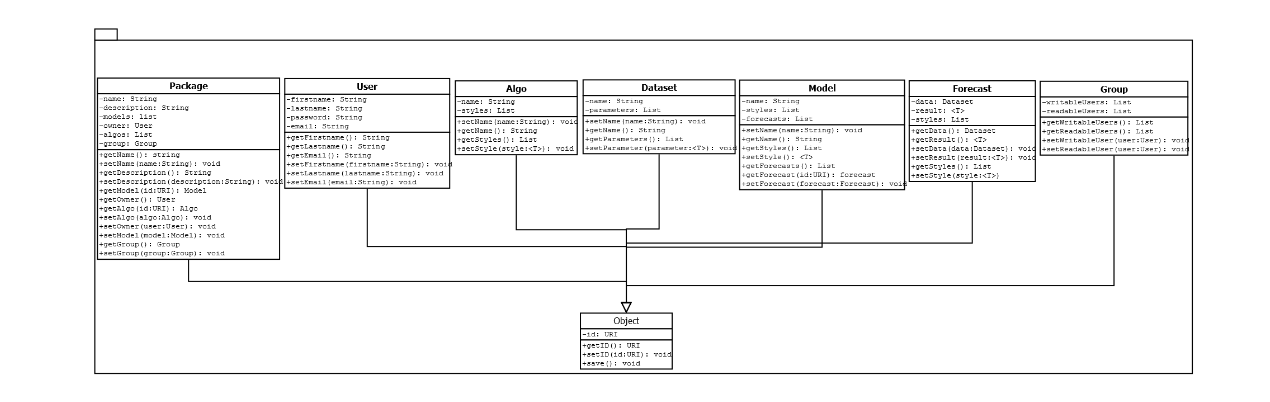
\includegraphics[scale=0.4]{Paket.png}
 	\caption{Das Paket mit den Klassen User, Model, Package, Dataset, Forecast, Group und Algo.}
 \end{figure}
 
 
\chapter{Client}

Der Client wird zum gro\ss{}en Teil mithilfe eines Model-View-Controller Patterns realisiert. Die verschiedenen View-Klassen stellen die Benutzeroberfläche des Clients dar. Der Controller bestimmt bei Forecast, Model und Algorithm die Art der Darstellung. Beispielsweise kann der Nutzer entscheiden, ob die Forecast als Baumdiagramm, Kurvendiagramm, o.\"a. ausgegeben wird. Selbiges gilt f\"ur die Models und Algorithmen. Bei Login und Admin haben die Controller die Aufgabe die m\"oglichen Eingaben zu verarbeiten oder zu verifizieren. 
 \begin{figure}[ht]
 	\centering
 	\includegraphics[scale=0.4]{Client.png}
 	\caption{Ausschnitt aus der Client Ebene.}
 \end{figure}



\chapter{Server}

Wir verwenden Apache Tomcat als Webserver, dieser enth\"alt ein Servlet-Container, mittels dessen wir mit dem Server kommunizieren. Als Datenbank verwenden wir eine RDF-Datenbank, diese wird durch Apache Jena TDB Triple-Store realisiert. 
Direkt unter den Servlets liegen die Interfaces der verschiedenen Objekte, dabei ist zu beachten, dass nur f\"ur Package, User und Group Manager n\"otig sind. Das liegt daran, dass die anderen Klassen (Model, Algo, Forecast und Dataset) \"uber die geerbten Methoden alle ben\"otigten Informationen, wie z.B. Packages abfragen k\"onnen. Um m\"ogliche Berechtigungen zu \"uberpr\"ufen kann in den Interfaces mit getCurrentUser der aktuelle Nutzer und somit auch seine Freigaben und Gruppen abgefragt werden.

Die Klassen ClientCrypter und ServerCrypter sind f\"ur die Ver- und Entschl\"usselung der Informationen zust\"andig. Somit k\"onnen keine Informationen direkt ausgelesen werden, falls Server und Client lokal voneinander getrennt sind. 
\begin{figure}[ht]
	\centering
	\includegraphics[scale=0.4]{server.png}
	\caption{Ausschnitt aus dem UML Diagramm f\"ur die Serverseite. Hinzukommen noch Klassen f\"ur Dataset, Group und Model}
\end{figure}



\chapter{Beispiel mit Sequenzdiagramm}

Im folgenden Sequenzdiagramm wird der Befehl 

\textit{\textless server \textgreater: \textless port \textgreater /package/ \textless id \textgreater /model/ \textless id \textgreater}  

\noindent dargestellt. Dabei versucht der eingeloggt Nutzer ein selbsterstelltes Model aufzurufen, auf das er die n\"otigen Rechte besitzt.

Dieser Vorgang wird realisiert, indem die Anfrage vom ModelIDServlet entgegen genommen wird. Das Interface ruft den PackageManager auf, der das Package von der Database anfordert. Nachdem das Package angefordert wurde, wird der owner des Packages mit Hilfe der checkRights Methode mit dem currentUser verglichen. Gibt es dort eine \"Ubereinstimmung, wird das Package an die oberen Schichten bis zum Client weitergegeben. 
\begin{figure}[ht]
	\centering
	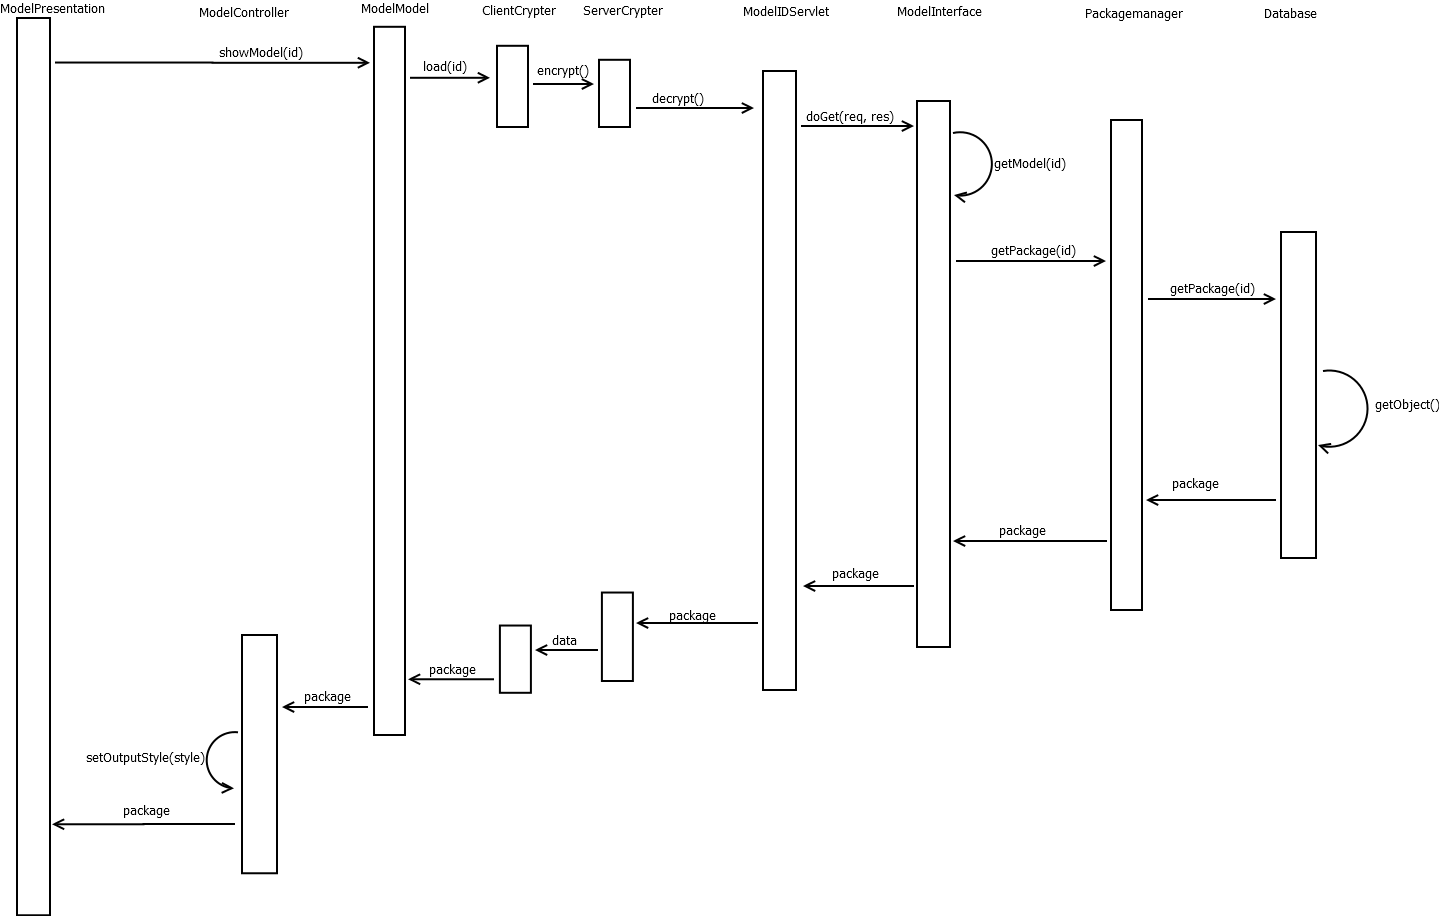
\includegraphics[scale=0.3]{sequenz.png}
	\caption{Sequenzdiagramm zum Aufrufen eines Models}
\end{figure}

\end{document}

%%% Local Variables:
%%% mode: latex
%%% TeX-master: t
%%% End:
































